\section{Proposed Gemini Design}
\label{sec:gemini-design}
%
% 1. give a 1-2 paragraph overview of the architecture
% 2. Create a subsection for each major component of the architecture
%       2-3 paragraph overview of component
%       parheads (with 2-3 paragarphs of content) for each design
%       choice/challenge/consideration.
% I imagine each subsection will be 1-2 columns.
%
% Throughout, point back to the use-caes, and comment on how they influence the
% design.

The Gemini design consists of a security policy specification and a monitor
that enforces the policy, both of which are transparent to applications.
%
The policy itself may aggregate rules from multiple, mutually
distrustful parties.
%
A prominent feature of the policy is that it allows for private data to be pinned
to specific trust domains, such as an organization's own machine.
%
The monitor manages the migration of an application's execution between domains
as the execution attempts to access pinned data, and ensures consistency of
resources shared between them.


Gemini's core abstraction is a \emph{distributed container},
where the filesystems and memory of the container may span several
domains, with each domain potentially cloaking parts of this space from the
others.
%
Each domain runs its own instance of the monitor, with the assumption that a
domain trusts its version of the monitor, but not those of its peers.
%
In an environment with trusted boot, where parties can attest to trusted peer
monitors, a party can augment a peer's monitor so as to enforce fine-grained
IFC rules to detect incorrect behavior during an application's execution.


We describe the three major aspects of Gemini's design: (1) the monitor, (2)
migration between domains, and (3) the security policy framework.
%
% The security policies are only interesting in the case of trusted monitors;
% otherise the policies are simply "to access object X, migrate to machine Y.
%
% Thus, I would descirbe the monitor and migration first with just that simple
% policy in mind, and then use the security policy section to describe the more
% interesting policies that trusted hardware allows.


\subsection{Monitors}
%
The monitor itself must simultaneously interpose on a process's execution while
also ensuring consistent policy enforcement for shared resources, such as files
and shared memory.
%
One approach is to base the design on full-system emulation.
%
However, full-system emulation is slow, as it needlessly emulates
monitored and unmonitored processes alike.
%
Moreover, previous
systems~\cite{whole-system-simulation,panorama,demand-emulation} that use this
technique in conjunction with taint tracking suffer from a lack of system
introspection, as well as the explosion of taint into kernel space.
%
Gemini's design instead takes a hybrid approach that splits the monitor between a
per-process monitor and a system monitor.



\parhead{Process monitor}
%
The process monitor is an emulator that instruments and dispatches the
application's code.
%
The emulator instruments instructions, such as
loads and stores, that propagate taint, as well as interposes on
system calls that transfer tainted data.
%
The process monitor tracks the propagation of taint in the process's
memory space using shadowed pages inaccessible to the application.
%

\parhead{System monitor}
The system monitor keeps a system-wide account of tainted resources,
ensures that processes are run in emulation mode when they have access to
tainted data, and applies policy checks over tainted data, such as when data is
emitted to the network.
%
To track taint through storage, the system monitor applies persistent
taint tags to files.
%
% Netlabel, CIPSO IETF draft
To transfer tainted buffers over the network, the system monitor embeds taint
tags in outging packets and processes tags from incoming packets.
%
In the case of untrusted boot, the policy that the system monitor enforces is
fairly simple: if a process attempts to access a page or a file pinned to
another domain, the monitor initiates a migration of execution to that domain.


\subsection{Execution migration}

Gemini migrates at the thread-level.
%
When a thread attempts to access a resource pinned to a target domain,
the system monitor suspends the thread, and transfers the
thread's execution to the target.
%
The thread runs on the target until it satisfies a \emph{migration condition},
and then migrates back to the source.
%
On return, the source updates the thread's context and the process's memory
space, and resumes the thread.


\parhead{Distributed Shared Memory}
%
Similar to prior systems, Gemini integrates distributed shared memory (DSM) and
virtual memory management.
%
Each domain runs a DSM manager and page server that cooperates with the VM
manager to service page faults.
%
The VM manager refers remote memory access to the DSM manager,
which in turn satifies the request using a coherence protocol with the peer
domain's page server.
%
Thus, a page fault to local memory is indistinguishable from a page fault to
remote memory.


\parhead{Distributed Filesystem}
%
Gemini maintains a consistent filesystem view among migrated and
non-migrated processes by allowing a thread's file descriptor table on the
target to proxy calls to a fileserver back on the source.
%
This has additional benefit of obviating the need to replicate or update
public files during migration.
%
Domains may pin file descriptors, such that the descriptor can only be used
in that domain.
%
Likewise, if the target thread writes tainted data to a remote descriptor, the
associated file transfers to, and becomes pinned by, the target; any processes
on source with that file open have subsequent operations on that descriptor
proxied to the target.


\parhead{Example: Loading a private key}
%
In Figure~\ref{fig:loading-key} we diagram a provider's service (source) loading
a private key pinned to the organization's machine (target).
%
We assume that the service is proprietary, and thus the provider
pins the custom portions of the software.
%
We assume that the service's cryptographic library is public, however.


In step 1, the source's monitor detects that one of the service's threads
attempts to open the cloaked key file.
%
The monitor suspends all the threads in the process, and transfers a minimal
subset of the thread's execution state to the target.
%
In step 2, the target monitor constructs a skeleton process and
restores the source's thread.
%
In restoring the thread, the target ensures that the only executable mappings
in the process correspond to the cryptographic library.
%
Likewise, during execution, the target's monitor will ensure that thread does
not create new executable mappings.


In step 3, the target resumes the thread in the process monitor's emulator,
tracking the propagation of the private key's data by adding taint tags to
the shadow table.
%
If the thread tries to access a page that the source has not yet tranferred,
the access generates a page fault.
%
The target's monitor traps such faults and redirects them to the source, which
responds with the faulted page.


When the process monitor detects a stopping condition, it notifies the
system monitor to suspend the thread and migrate back to the source machine.
%
The stopping condition is policy-specific; examples include the process
performing $n$ consecutive instructions without tainted
data, or the instruction pointer referencing source-cloaked data or code.
%
In step 4, the source's system monitor updates it's memory mappings based on
the target's exeuction, and sets page table attributes to indicate which pages
are now cloaked by the target.
%
As with the migration to the target, the source must also perform consistency
checks.
%
The source then resumes the threads.


\begin{figure}[t]
	\centering
    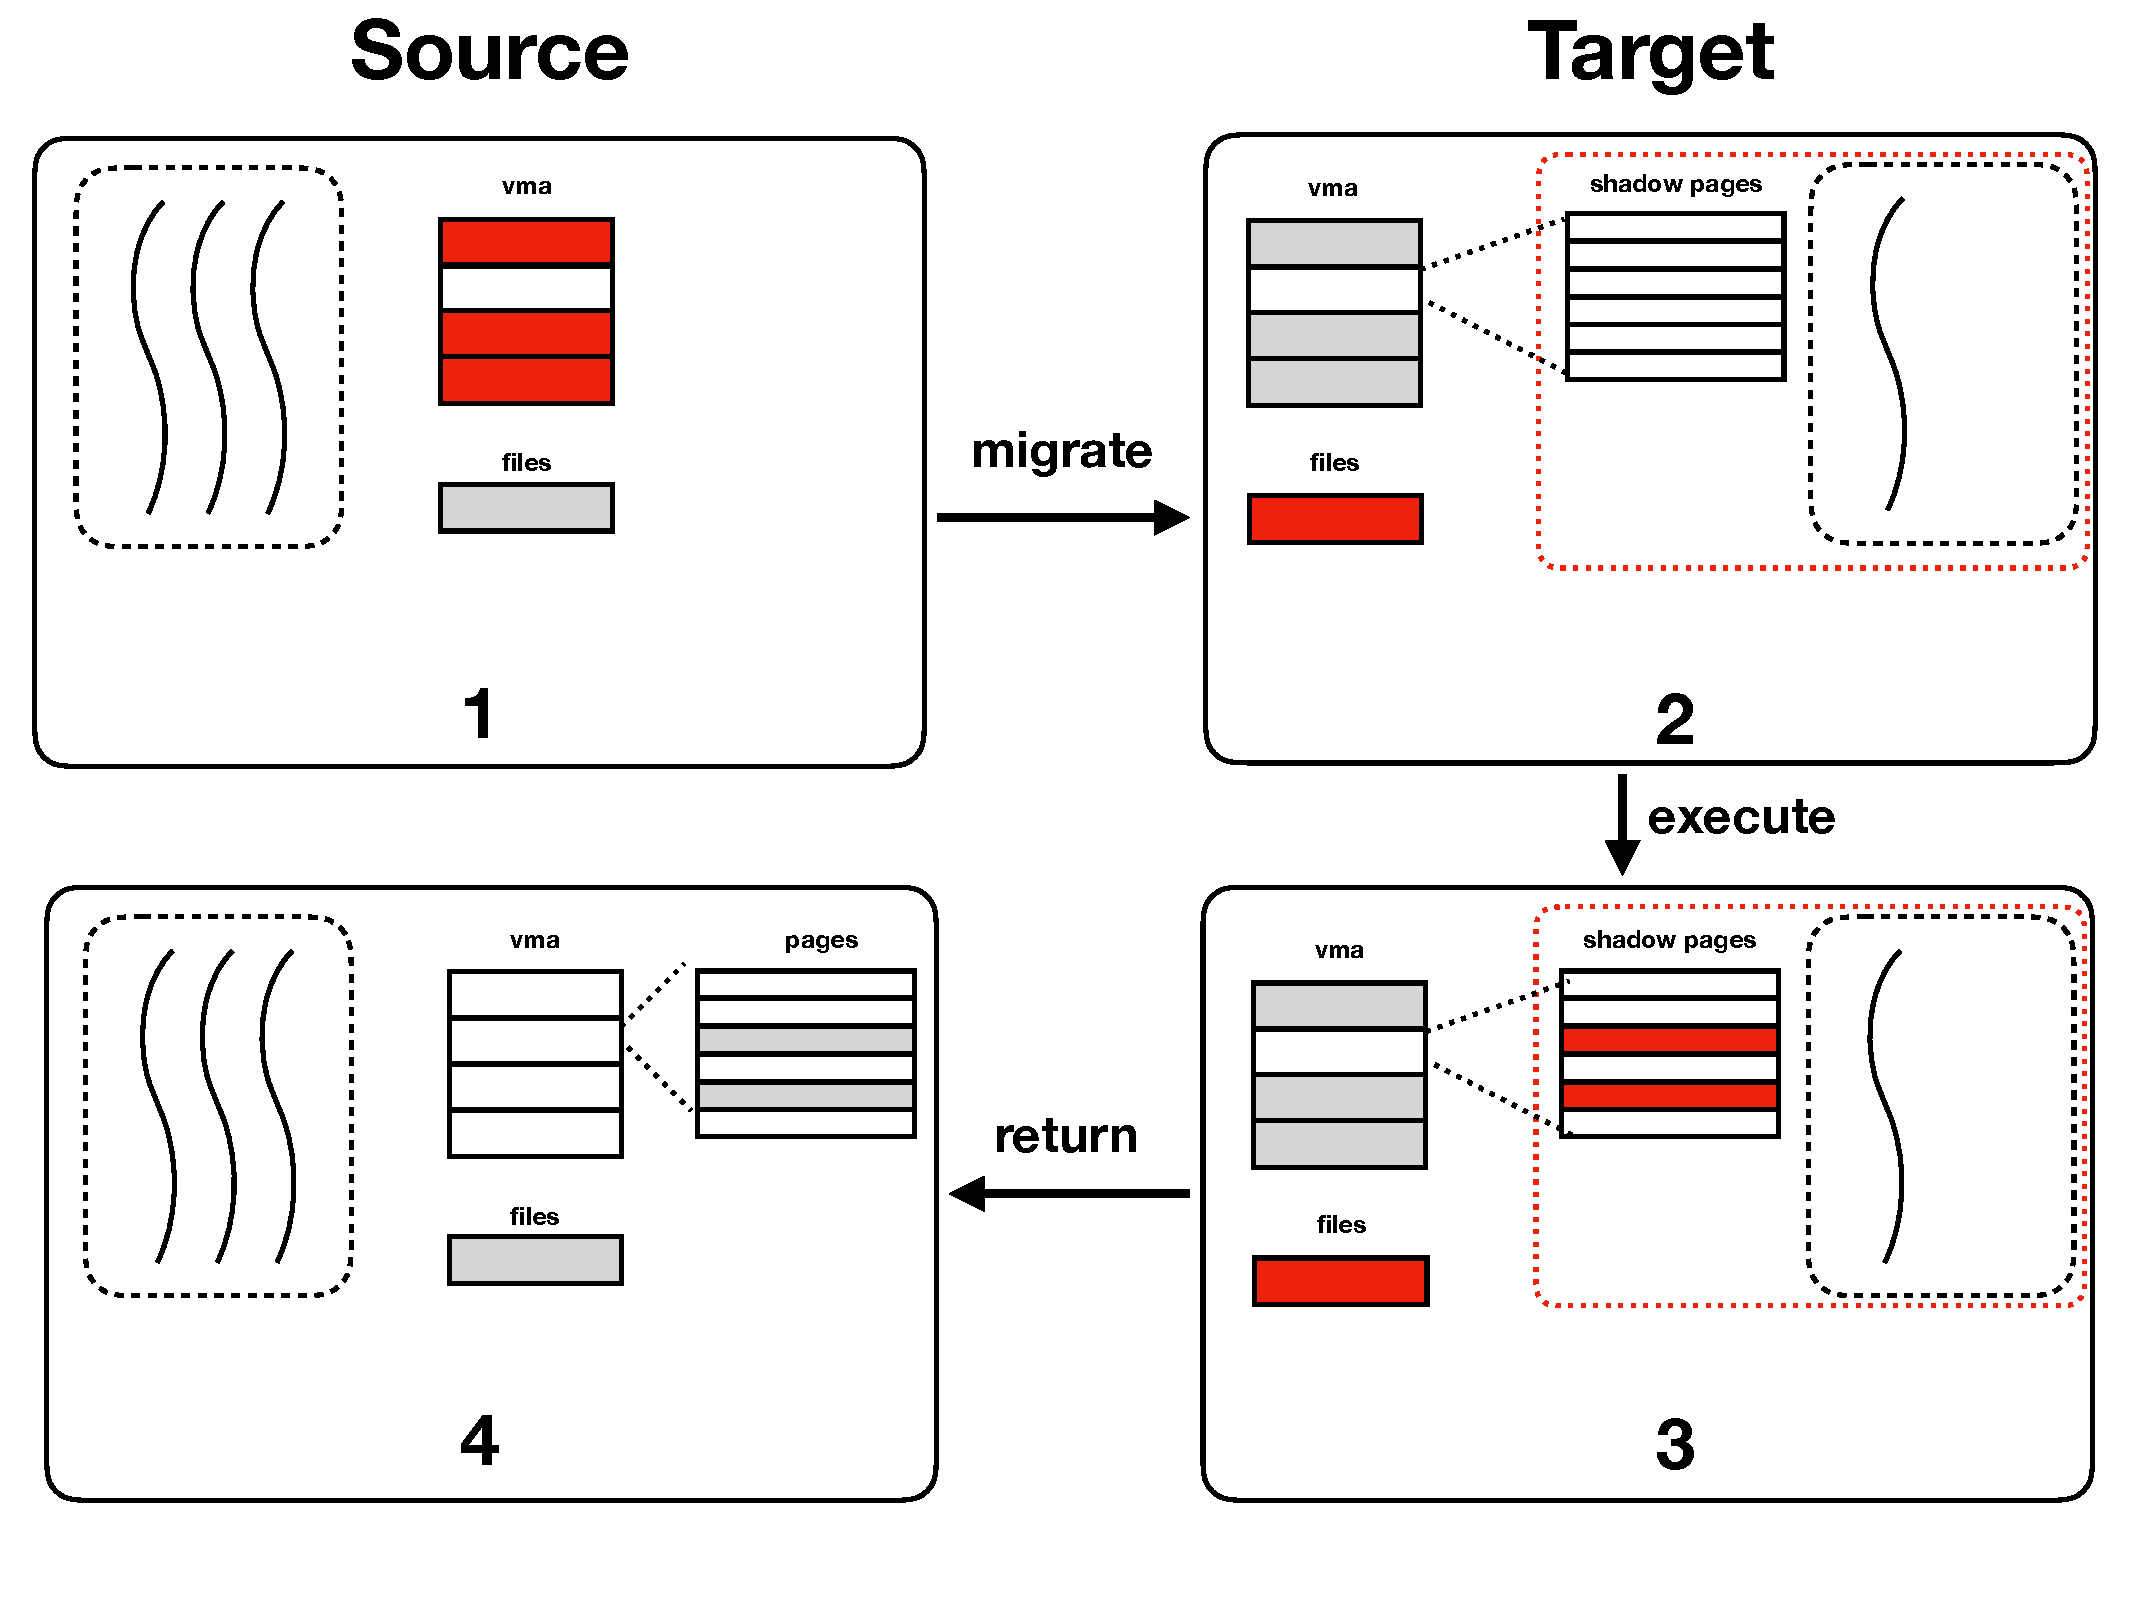
\includegraphics[width=0.5\textwidth]{figs/loading-key}
	%
    \caption{A webserver on the service provider's domain (source) loading a
    private key pinned to the organization's domain (target).
    %
    Cloaked virtual memory areas (VMAs) an files are in gray, and pinned
    resources are in red.
    }
	%
	\label{fig:loading-key}
\end{figure}


\parhead{Example: Signing operation}
%
Migration for a signing operation is similar to that for loading a
private key.
%
For signing, however, the source's monitor detects an 
access attempt to pinned data via a page fault for the cloaked memory page
storing the key.
%
When the thread, executing on the target, computes the signature, the target's
monitor must also specify a \emph{declassification gate} to remove the taint that
would otherwise pin the signature to the target.
%
In this example, the gate is a ``hook"  for the cryptographic library's
signing function.
%
With declassification gates, the target must guard against attempts by the source to
hijack declassification.
%
For instance, the source could arrange for the thread to be restored with a
starting point that invokes \texttt{sign(0, key}), thereby declassifying the key.
%
Thus, the target must properly sanitize a gate's arguments.


\parhead{Limitations}
% TODO:DSM and test-and-set?
%
A disadvantage of the integration between VM and DSM is that the unit of access
adn locking are contrainted to be a page.
%
If multiple data structures are allocated on the same page, then this constaint
can lead to \emph{false sharing}, wherein distinct private data structures
appear shared due to colocation on the same page.
%
A similar issues exists with applying taint tags at the page granularity.


Gemini is also susceptible to a form of deadlock whereby, during the course of
a thread's execution, the thread reaches an instruction that accesses two
pieces of data, each pinned to a separate domain.
%
We simply specify that Gemini must detect such occurences and abort.


In our uses-cases, this form of deadlock is either non-existent or unusual, as
only a single party has pinned data, or the pinned data of each party is used 
in logically different portions of the code (e.g., an email provider pinning
proprietary spam rules, and an organization pinning a private key).
%
A more plausible deadlock scenario is a server that supports multiple tenants
and uses a global data structure to manage the (pinned) keys across all
tenants.
%
In such cases, the application may need to be patched to correct the offending
memory layout.
%
In the general case, the problem is one of secure multi-party computation, and
an interesting area of future work is for the emulator to emit garbaled
circuits when it detects such events.


\subsection{Security policies}
%
There are two types of security policies: \emph{confidentiality policies} and
\emph{integrity policies}.
%
Confidentiality policies either pin data or restrict the accesss privileges of
code with respect to the data.
%
Integrity policies specificy a service's behavior
based on the flow of the data within and from that service. 


Policies are expressed over taint tags.
%
A tag belongs to one of three classes: \emph{pinned}, \emph{provenance},
or \emph{access}.
%
A pinned tag applies to code and data, and indicates the domain (such
as a host) that has pinned the associated code or data.
%
A provenance tag applies only to data and indicates that either a domain or a piece of
code has processed that data.
%
An access tag applies to domains, code, and data, and indicates the read or
write privileges of the domain or code with respect to the data.


Organizations introduce tags into the system by either a tool (or monitor) that
tags static files, or by egress rules that tag data as it transfers from
between domains.
%
Monitors propagate the tags in accordance with computation across the memory
space, filesystem, and network.


\parhead{Confidentiality Policies}
\begin{enumerate}
    \item[C1]  The organization's private key(s) must not be leaked to untrusted parties.
\end{enumerate}


\parhead{Integrity Policies}

\begin{enumerate}
    \item[I1] If the organization's data (e.g., webpage, DNS records, emails) leaves the
        service, it must be sent over a flow endorsed by the organization's private
        key.

    \item[I2] Any flow endorsed by the organization's private key must only send
        data originating from the organization.

    \item[I3] If the organization's data leaves the service, it must not have been
        modified.
\end{enumerate}

Policies (I2) and (I3) are impractically strict: web and mail servers will add
headers to the outgoing content, and may further modify the content through a
legitimate transformation, such as compression or image transcoding.
%
Thus, these assertions may give rise to additional qualificaitons.
%
For instance, to allow for server-provided headers, assertion (3) may instead
be specified as: ``Any flow endorsed by the organization's private key must
\emph{eventually} send data originating from the organization."


\parhead{Transitive Closure Policy}

\begin{enumerate}
    \item In the case of a distributed service, the organization's data can
        traverse other nodes that  guarantee the above properties.
\end{enumerate}


% The TLS frames will contain metadata fields (sequence numbers, etc.),
% that are not tagged as belonging to the organization.
% %
% Thus, the monitor uses an application-layer parser to parse the
% messages, and consults with the policy regarding which tags should be on
% which fields.
% %
% If simple temporal logic is fine (not labeled until labeled), then the monitor
% does need the underlying plaintext; otherwise, the monitor must further impose
% an implementation requirements on the application; namely, the use of
% kernel-TLS\@.


\parhead{Example: HTTPS Edge Server}
%
Execution migrates to the organization, which produces an RSA signature, and
then execution migrates back to the CDN\@.
%
Before migrating back to the CDN, the organization assigns a taint tag to the
signature, which is also sent to the CDN\@.
%
The CDN sends the signature to a web client as part of the ServerHello TLS
message.
%
When the CDN's monitor sends the signature, it marks the corresponding flow
with the tag.


If the client requests a web page that is not in the server's cache, the server
makes an HTTPS request to the organization's origin server and downloads the
page.
%
The CDN's monitor detects that the request is made to the origin and tags the
downloaded page to indicate its provenance (alternatively, the origin server
could embed these tags in its response packets).
%
When the CDN sends the page to the client over subsequent TLS frames the
monitor checks that these frames include data that is tagged as originating
from the organization. 


\begin{figure}[t]
	\centering
    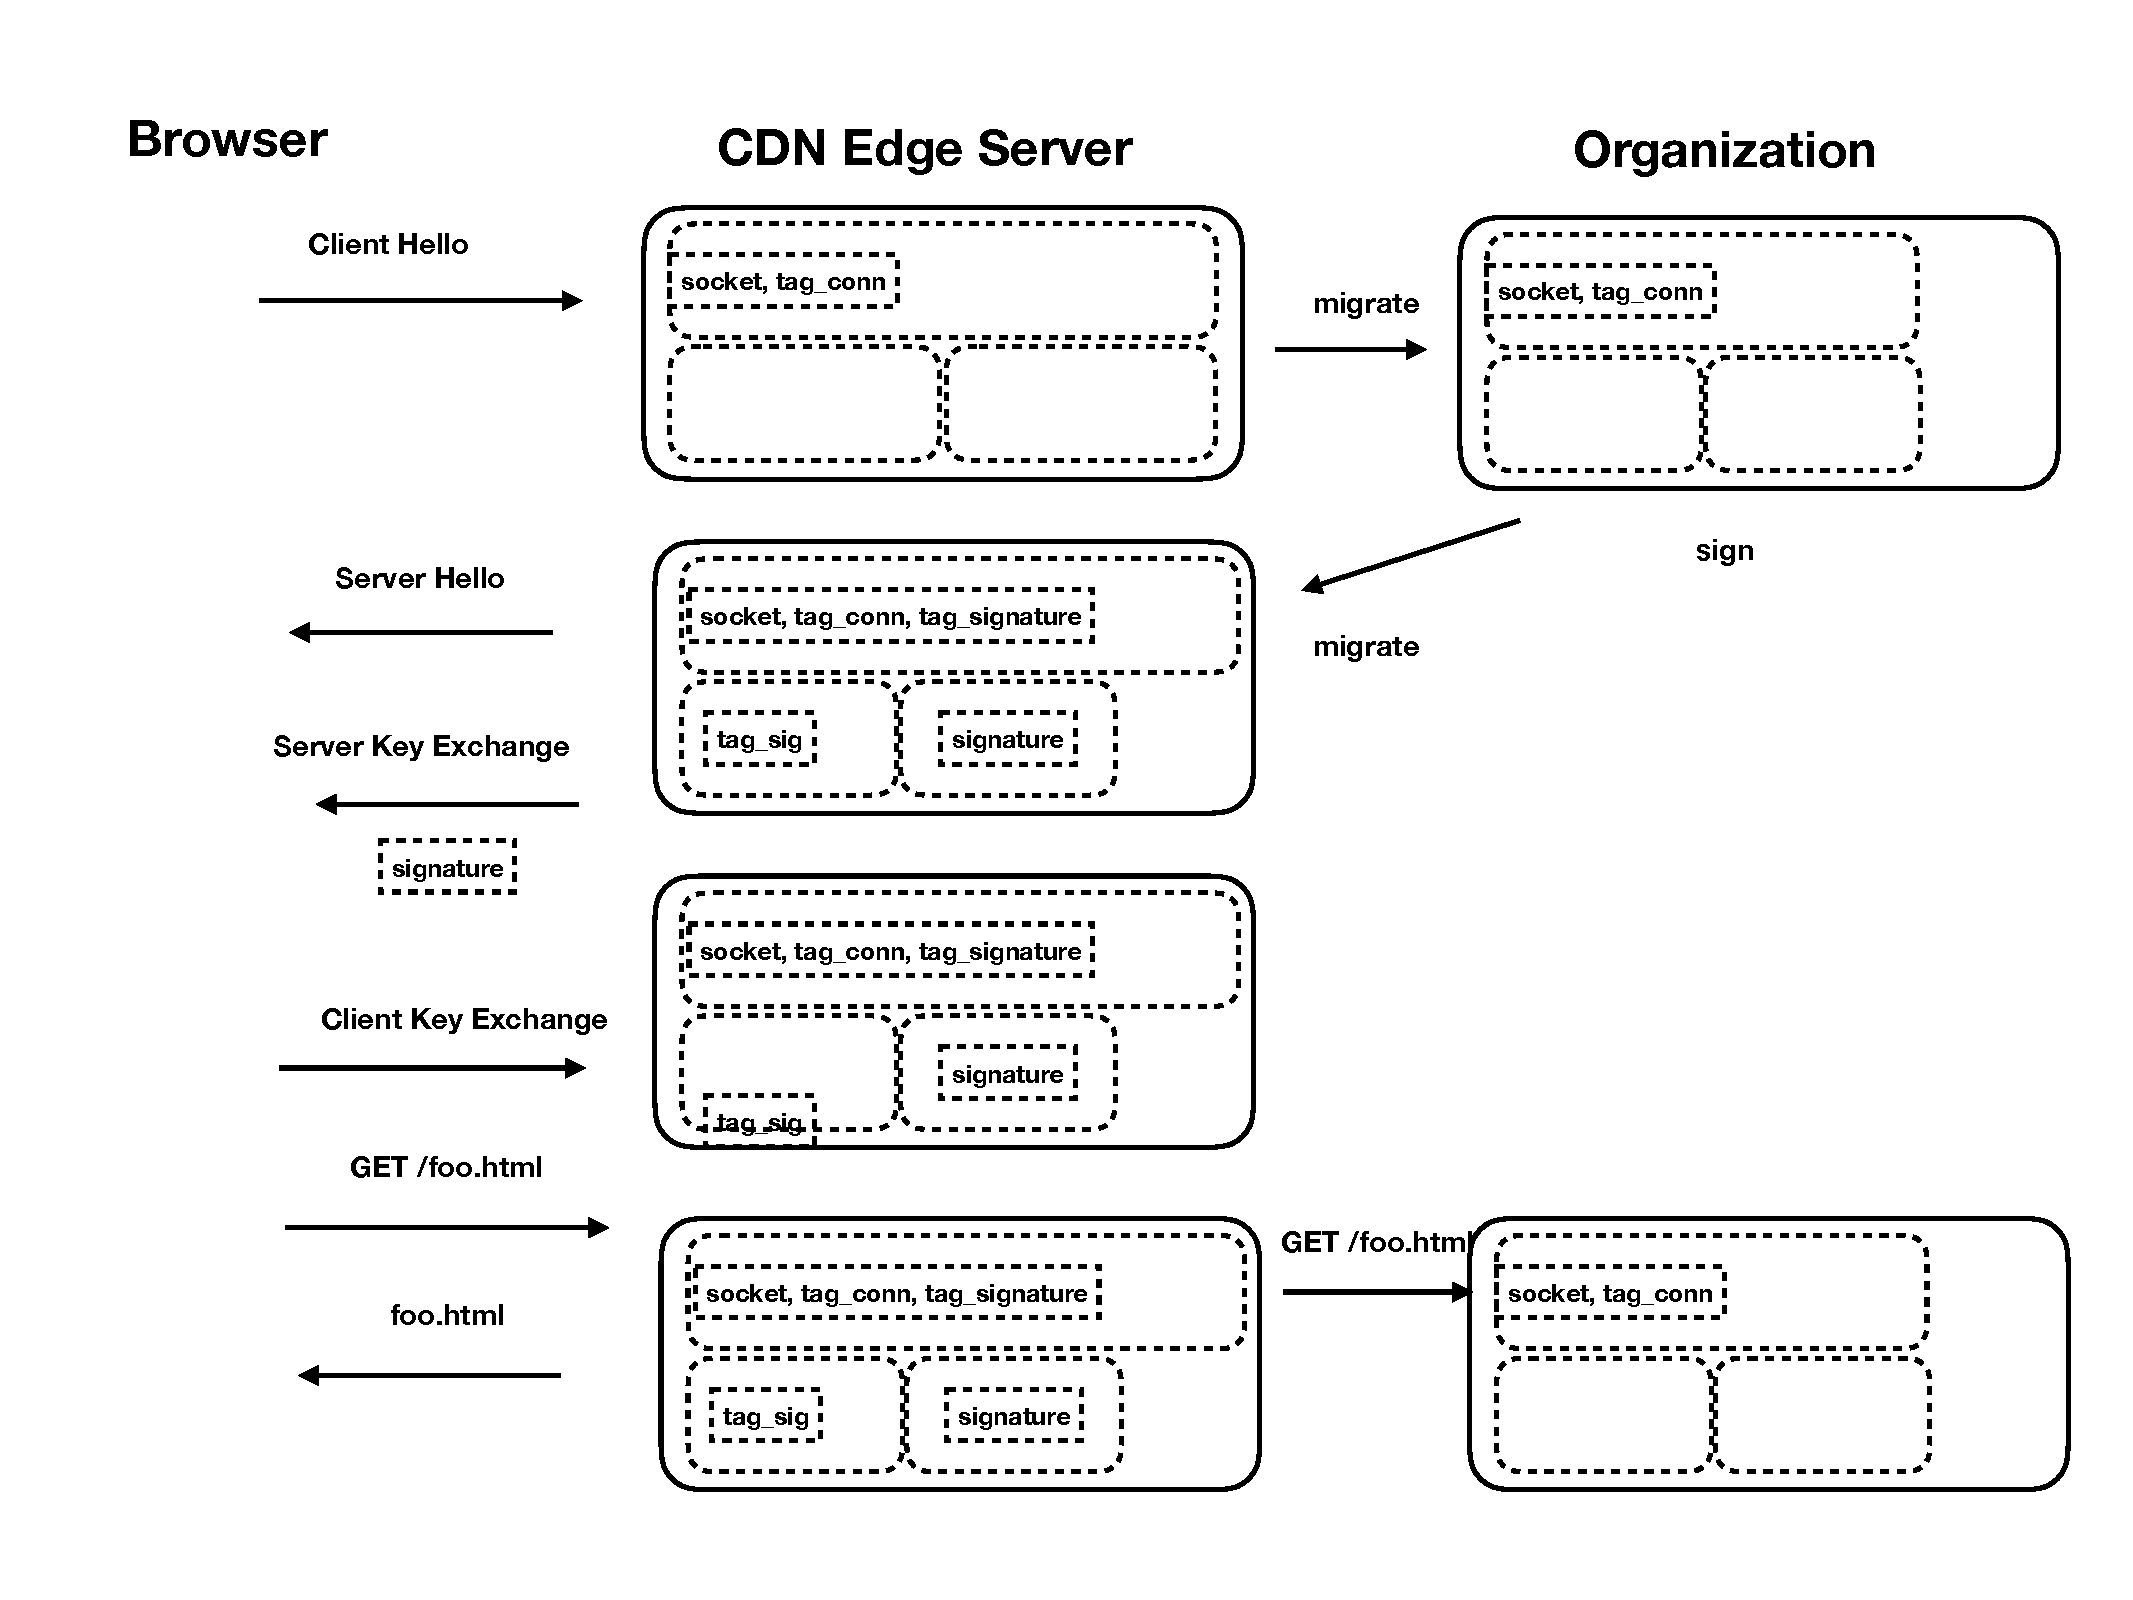
\includegraphics[width=0.5\textwidth]{figs/https-flowchart}
	%
    \caption{The evalution of taint-based firewall rules for an HTTPS proxy
    service.}
	%
	\label{fig:https-flowchart}
\end{figure}


% \parhead{Application: DNS Authoritative Server}
% %
% The firewall rules for a DNSSEC-enabled server inspects incoming packets, and keep a
% running mapping of the requests's ID to whether the request requires DNSSEC
% (the request's \texttt{DO} bit).
% %
% When sending responses, the policy  parses the response's ID and retrieves the
% corresponding \texttt{DO} value from the mapping.
% %
% If the mapping indicates that the request set \texttt{DO}, the firewall
% verifies that the response includes an \texttt{RRSIG} record tagged with the
% organization's private key.
% %
% Regardless, the firewall verfiies that the remaining response data is tagged as originating
% from the organization.


\parhead{Tag Properties}
%
\begin{widelist}
\item \textbf{Unforgeable:}
    %
    A possible attack is that the provider adds its own policy that taints data as
    if it came from the organization, and so the data passes the organization's
    policy monitor.
    %
    This threat implies that either the monitors maintain the secrecy of the tags
    from the untrusted applications, or make them unforgeable.
    %
    The problem with maintaining tag secrecy is that tags may appear as metadata
    attached to files and stream.

\item \textbf{Irrevocable:}
    %
    If Gemini is running in a secure enclave, organization $A$ might apply
    a tag to its enclaved private key that specifies that only a specific
    piece of code is allowed to access the data.
    %
    Thus, it is necessary that organization $B$ be unable to remove $A$'s tag,
    lest $B$ gain access to $A$'s private key.
    %
    In short, only an organization can remove its own tags.

\item \textbf{Multiple tags per byte:}
    %
    As shown by the two examples above, there is need for the system to support
    assigning multiple tags to a given byte.

\item \textbf{Multiple tags per organization:}
    %
    As shown by the two examples above, there is need for the system to support
    assigning multiple tags from the same organization.

\item \textbf{Large tag space:}
    %
    Due to an HTTPS or DNS server simultaneously hosting many tenants, the
    system most support a large tag space.
\end{widelist}

For space considerations, there may also be the need to perform tag coalescing, as where
many contiguous bytes share the same tag set.


\parhead{Egress Monitor}
%
Egress monitors are primarily for integrity, not confidentiality, and thus
we do not have to be concerned with the monitor laundering taint.
%
Egress monitors perform two tasks: (1) request attestations from remote
monitors, and (2) provide a mechanisms for stateful, tag-aware, packet filters.
%
One challenge is that the packet filters may have to operate over encrypted
data, which might diffuse the taint applied to the underlying plaintext.
%
In such cases, I  envision the monitor must imposing
an implementation requirement on the application; namely, the use of
kernel-TLS\@.
%
An additiona design contraint regarding performance is that, in the case of
multi-tenancy, a system may have many egress policies that are identical with
the exception of the tag values.  Thus, I might have a monitor-level policy
whereby monitors can only view data that includes one of its tags.




% How does tagging code work?
%   You could tag openssl with the a tag from the org that grants openssl
%   permission.
%
%   You could assume that openssl is tagged by openssl's org, and the data's
%   tag specifiies who can read it.
%
%   These seem pretty much the same to me.
%
%       You don't want to have to run the origin server under emulation --
%       it's not doing any taint tracking.  So, instead, you can imagine 
%       applying the taint at the network filter.
%
